\subsection{Pruebas de la versión: 3} \label{chp:pruebasV3}
En esta sección se describen los resultadods de las pruebas realizadas de la tercera versión del algoritmo de optimización de horarios.\\

Como consideración tenemos que las pruebas fueron realizadas en una laptop dell Inspiron 15 con procesador intel i5 5ta generación 4gb de memoria ram usando el sistema operativo debian 9.\\


\subsubsection{Pruebas realizadas}

Inicialmente las funciones que comprenden el algoritmo fueron probadas por separado. \\

\begin{itemize}
	\item Se corroboró que la función de generar Población utilizara todas las opciones de Materia-Profesor disponibles y que el resultado tuviera la estructura que hemos definido. 
	
	\item Se probó la función de evaluación, para corroborar que las restricciones ingresadas sean tomadas en cuenta al momento de asignar una calificación a un horario.
	
	\item Se probaron las funciones de mutación de forma que el resultado arrojado después de llevar a cabo dichos operadores sea en realidad distinto a la entrada del mismo así como se corroboró que se llevaran a cabo de la manera esperada.
	
\end{itemize}

Una vez que se corrigieron los errores arrojados por las pruebas de la versión 2 del algoritmo, se adaptó el segundo prototipo de manera que la función principal reciba como parámetros, el número de iteraciones que se van a realizar, el número de individuos que conforman la población inicial y el número de estructuras educativas que el actor desea como resultado del algoritmo. Para corroborar que el funcionamiento fuera correcto, utilizamos la estructura educativa actual de la ESCOM para el nivel 2 y el turno matutino. Utilizando estos datos y teniendo en cuenta los resultados de las pruebas del prototipo 2, se realizó una experimentación para determinar el tamaño óptimo de la población inicial.\\

En una junta con el profesro Iván Giovanny Mosso, se le cuestionó sobre el número de estructuras educativas que le gustaría tener disponibles para analizar cuál es la mejor opción a lo que respondió 5, de esta manera para asegurarnos de que este requerimiento se satisfaga y siga siendo sostenible a futuro, determinamos permitir que se solicite al sistema arrojar un máximo de 10 estructuras educativas, de esta manera las pruebas fueron llevadas a cabo considerando el número máximo posible de estructuras educativas deseadas como resultado.\\

El tamaño de la población inicial influye de manera directa en el aumento tiempo que tarda en ejecutarse el algoritmo, sin embargo de igual manera influye en la disminución del número de iteraciones requeridas para lograr 10 estrucutras educativas. En cinco ocasiones se tomó el número de iteraciones que toma al algoritmo encontrar 10 posibilidades de estructura educativa con calificación óptima para cada uno de los tamaños probados para la población inicial. En la figura \ref{fig:PruebaV3} se muestran los resultados del experimento y en la figura \ref{fig:grafV3} se muestra la gráfica de los mismos donde se puede apreciar que el número iteraciones disminuye conforme el tamaño de la población inicial aumenta, sin embargo también se puede observar en la tabla el aumento en el tiempo. De esta manera se determinó que el punto medio entre el aumento de tiempo y la disminución de las iteraciones debe ser tomado como el mejor para nuesto algoritmo por lo que se tomó un tamaño de la población inicial de 30 individuos.\\
 
 \begin{figure}[htbp!]
 	\begin{center}
 		\fbox{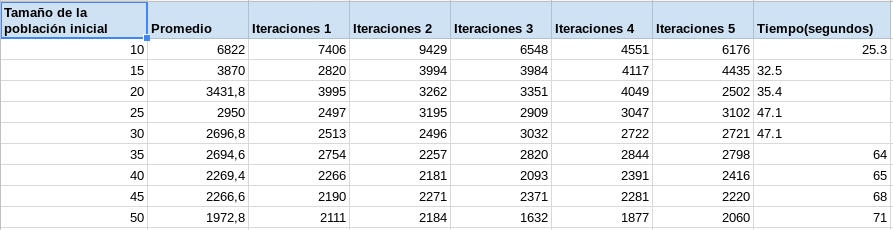
\includegraphics[width=.7\textwidth]{ModeloComportamiento/Algoritmo/imagenes/tabla3.png}}
 		\caption{Determinación experimental del criterio de paro}
 		\label{fig:PruebaV3}
 	\end{center}
 \end{figure}


\begin{figure}[htbp!]
	\begin{center}
	\fbox{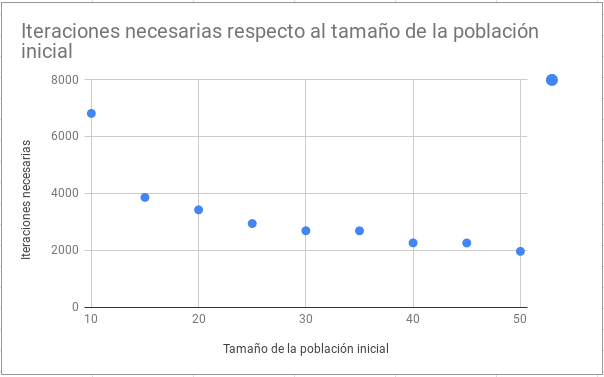
\includegraphics[width=.7\textwidth]{ModeloComportamiento/Algoritmo/imagenes/grafica3.png}}
		\caption{Gráfica de mejora}
		\label{fig:grafV3}
	\end{center}
\end{figure}

